Project made using QT Creator in C++\hypertarget{index_about}{}\section{About}\label{index_about}
A simple cross-\/platform steganography project which hides data in images. This project is built using M\+VC pattern and features G\+UI. \href{https://qt.io}{\tt Qt} and \href{https://github.com/bricke/Qt-AES}{\tt Q\+A\+E\+S\+Encryption} by \href{https://github.com/bricke}{\tt bricke} were used. You can read more about project at the \href{../}{\tt home page}\hypertarget{index_structure}{}\section{Structure of the project}\label{index_structure}
As written earlier this project is structured with M\+VC pattern. Here is a small graph showing the basic structure. 
\begin{DoxyImageNoCaption}
  \mbox{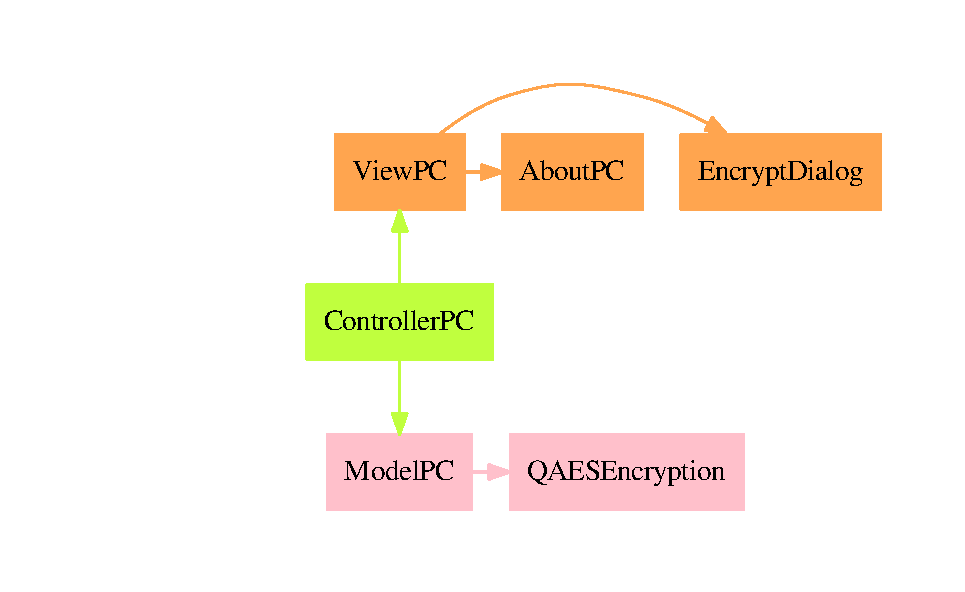
\includegraphics[width=\textwidth,height=\textheight/2,keepaspectratio=true]{dot_structure}}
\end{DoxyImageNoCaption}
\hypertarget{index_ext-use}{}\section{ext-\/use}\label{index_ext-use}
You can use \hyperlink{class_model_p_c}{Model\+PC} class separately from View and Control layer. You will need four files\+: \hyperlink{modelpc_8cpp}{modelpc.\+cpp} \hyperlink{modelpc_8h}{modelpc.\+h} \hyperlink{qaesencryption_8cpp}{aes/qaesencryption.\+cpp} \hyperlink{qaesencryption_8h}{aes/qaesencryption.\+h}

Then you can just {\ttfamily \#include \char`\"{}modelpc.\+h\char`\"{}} and use A\+PI.